\documentclass[11pt,a4paper]{report}

% =============================================================================
% PREAMBLE: Packages and Dark Theme Configuration
% =============================================================================

% Core packages
\usepackage[utf8]{inputenc}
\usepackage[T1]{fontenc}
\usepackage{lmodern}
\usepackage[margin=1in]{geometry}
\usepackage{graphicx}
\usepackage{amsmath,amssymb,amsfonts}
\usepackage{booktabs}
\usepackage{array}
\usepackage{tabularx}
\usepackage{longtable}
\usepackage{hyperref}
\usepackage{cleveref}
\usepackage{enumitem}
\usepackage{fancyhdr}
\usepackage{titlesec}
\usepackage{tocloft}
\usepackage{parskip}

% Color and dark theme
\usepackage{xcolor}

% Define dark theme colors
\definecolor{bgcolor}{HTML}{1e1e1e}        % Dark slate background
\definecolor{textcolor}{HTML}{d4d4d4}      % Off-white text
\definecolor{headingcolor}{HTML}{569cd6}   % Soft blue for headings
\definecolor{accentcolor}{HTML}{4ec9b0}    % Teal accent
\definecolor{linkcolor}{HTML}{ce9178}      % Warm link color
\definecolor{codebackground}{HTML}{2d2d2d} % Slightly lighter for code
\definecolor{codekeyword}{HTML}{c586c0}    % Purple keywords
\definecolor{codestring}{HTML}{ce9178}     % Orange strings
\definecolor{codecomment}{HTML}{6a9955}    % Green comments
\definecolor{codenumber}{HTML}{b5cea8}     % Light green numbers

% TikZ colors for diagrams
\definecolor{blockfill}{HTML}{3c3c3c}
\definecolor{blockborder}{HTML}{569cd6}
\definecolor{signalcolor}{HTML}{4ec9b0}
\definecolor{datacolor}{HTML}{dcdcaa}
\definecolor{controlcolor}{HTML}{c586c0}
\definecolor{memorycolor}{HTML}{ce9178}

% Apply dark theme
\pagecolor{bgcolor}
\color{textcolor}

% Hyperref configuration
\hypersetup{
    colorlinks=true,
    linkcolor=linkcolor,
    urlcolor=accentcolor,
    citecolor=accentcolor,
    pdftitle={LDC FPGA Hardware Implementation: Technical Reference Manual},
    pdfauthor={VLSI Design Team},
}

% Code listings
\usepackage{listings}

\lstdefinestyle{darkstyle}{
    backgroundcolor=\color{codebackground},
    basicstyle=\ttfamily\small\color{textcolor},
    keywordstyle=\color{codekeyword}\bfseries,
    stringstyle=\color{codestring},
    commentstyle=\color{codecomment}\itshape,
    numberstyle=\tiny\color{codenumber},
    numbers=left,
    numbersep=8pt,
    breaklines=true,
    breakatwhitespace=false,
    tabsize=4,
    showspaces=false,
    showstringspaces=false,
    frame=single,
    framerule=0.5pt,
    rulecolor=\color{blockborder},
    xleftmargin=15pt,
    framexleftmargin=15pt,
    aboveskip=10pt,
    belowskip=10pt,
}

\lstdefinelanguage{Verilog}{
    morekeywords={module,endmodule,input,output,wire,reg,always,begin,end,
                  if,else,case,endcase,for,while,assign,posedge,negedge,
                  parameter,localparam,integer,signed,function,endfunction,
                  task,endtask,initial,fork,join},
    sensitive=true,
    morecomment=[l]{//},
    morecomment=[s]{/*}{*/},
    morestring=[b]",
}

\lstdefinelanguage{Python}{
    morekeywords={def,return,if,else,elif,for,while,import,from,as,class,
                  True,False,None,and,or,not,in,is,with,try,except,finally,
                  raise,assert,yield,lambda,pass,break,continue,global},
    sensitive=true,
    morecomment=[l]{\#},
    morestring=[b]",
    morestring=[b]',
}

\lstset{style=darkstyle}

% TikZ for diagrams
\usepackage{tikz}
\usetikzlibrary{positioning,arrows.meta,shapes.geometric,shapes.multipart,
                fit,calc,backgrounds,decorations.pathreplacing,matrix}

% TikZ styles for dark theme diagrams
\tikzset{
    block/.style={
        rectangle,
        draw=blockborder,
        fill=blockfill,
        text=textcolor,
        minimum height=1cm,
        minimum width=2.5cm,
        align=center,
        rounded corners=2pt,
        line width=0.8pt,
    },
    smallblock/.style={
        rectangle,
        draw=blockborder,
        fill=blockfill,
        text=textcolor,
        minimum height=0.7cm,
        minimum width=1.8cm,
        align=center,
        rounded corners=2pt,
        line width=0.6pt,
        font=\small,
    },
    memblock/.style={
        rectangle,
        draw=memorycolor,
        fill=blockfill,
        text=textcolor,
        minimum height=1cm,
        minimum width=2cm,
        align=center,
        line width=0.8pt,
    },
    signal/.style={
        ->,
        >=Stealth,
        line width=0.8pt,
        signalcolor,
    },
    data/.style={
        ->,
        >=Stealth,
        line width=1pt,
        datacolor,
    },
    control/.style={
        ->,
        >=Stealth,
        line width=0.6pt,
        controlcolor,
        dashed,
    },
    bus/.style={
        ->,
        >=Stealth,
        line width=1.5pt,
        datacolor,
    },
    label/.style={
        text=textcolor,
        font=\footnotesize,
    },
    register/.style={
        rectangle,
        draw=accentcolor,
        fill=blockfill,
        text=textcolor,
        minimum height=0.6cm,
        minimum width=1.2cm,
        align=center,
        line width=0.6pt,
        font=\small,
    },
}

% Heading formatting
\titleformat{\chapter}[display]
    {\normalfont\huge\bfseries\color{headingcolor}}
    {\chaptertitlename\ \thechapter}{20pt}{\Huge}
\titleformat{\section}
    {\normalfont\Large\bfseries\color{headingcolor}}
    {\thesection}{1em}{}
\titleformat{\subsection}
    {\normalfont\large\bfseries\color{accentcolor}}
    {\thesubsection}{1em}{}
\titleformat{\subsubsection}
    {\normalfont\normalsize\bfseries\color{textcolor}}
    {\thesubsubsection}{1em}{}

% Table of contents styling
\renewcommand{\cftchapfont}{\color{headingcolor}\bfseries}
\renewcommand{\cftsecfont}{\color{textcolor}}
\renewcommand{\cftsubsecfont}{\color{textcolor}}
\renewcommand{\cftchapleader}{\color{textcolor}\cftdotfill{\cftdotsep}}
\renewcommand{\cftsecleader}{\color{textcolor}\cftdotfill{\cftdotsep}}
\renewcommand{\cftchappagefont}{\color{headingcolor}}
\renewcommand{\cftsecpagefont}{\color{textcolor}}

% Header/footer
\pagestyle{fancy}
\fancyhf{}
\fancyhead[L]{\color{textcolor}\leftmark}
\fancyhead[R]{\color{textcolor}\thepage}
\fancyfoot[C]{\color{textcolor}\footnotesize LDC FPGA Implementation -- Technical Reference}
\renewcommand{\headrulewidth}{0.4pt}
\renewcommand{\headrule}{\hbox to\headwidth{\color{blockborder}\leaders\hrule height \headrulewidth\hfill}}

% Custom commands
\newcommand{\qformat}[1]{\texttt{\color{accentcolor}#1}}
\newcommand{\signal}[1]{\texttt{\color{datacolor}#1}}
\newcommand{\state}[1]{\texttt{\color{codekeyword}#1}}
\newcommand{\regname}[1]{\texttt{\color{memorycolor}#1}}

% =============================================================================
% DOCUMENT BEGIN
% =============================================================================

\begin{document}

% -----------------------------------------------------------------------------
% TITLE PAGE
% -----------------------------------------------------------------------------

\begin{titlepage}
    \centering
    \vspace*{2cm}
    
    {\Huge\bfseries\color{headingcolor} LDC FPGA Hardware Implementation\par}
    \vspace{0.5cm}
    {\LARGE\color{accentcolor} Technical Reference Manual \& Design Document\par}
    
    \vspace{1.5cm}
    
    {\large\color{textcolor} Lightweight Dense CNN for Edge Detection\par}
    {\large\color{textcolor} Custom RTL Implementation through \texttt{ldc\_block2}\par}
    
    \vspace{2cm}
    
    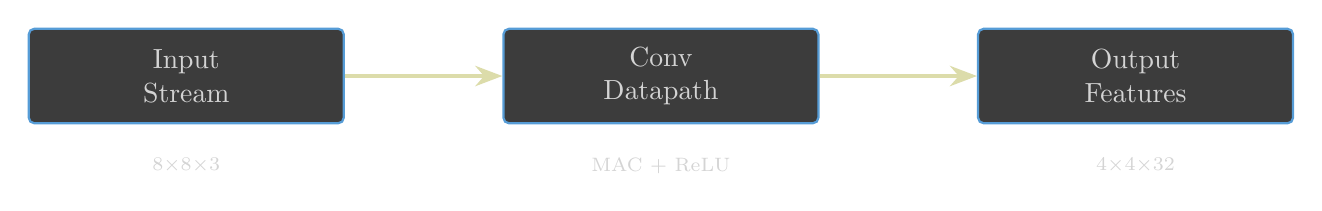
\begin{tikzpicture}
        \node[block, minimum width=4cm, minimum height=1.2cm] (input) {Input\\Stream};
        \node[block, minimum width=4cm, minimum height=1.2cm, right=2cm of input] (conv) {Conv\\Datapath};
        \node[block, minimum width=4cm, minimum height=1.2cm, right=2cm of conv] (output) {Output\\Features};
        
        \draw[bus] (input) -- (conv);
        \draw[bus] (conv) -- (output);
        
        \node[below=0.3cm of input, label, font=\scriptsize] {8$\times$8$\times$3};
        \node[below=0.3cm of conv, label, font=\scriptsize] {MAC + ReLU};
        \node[below=0.3cm of output, label, font=\scriptsize] {4$\times$4$\times$32};
    \end{tikzpicture}
    
    \vfill
    
    {\large\color{textcolor} Core Datapath, DSP Math, and Digital Logic\par}
    \vspace{0.5cm}
    {\normalsize\color{codecomment} Scope: Through \texttt{ldc\_block2} verification\par}
    
    \vspace{1cm}
    
    {\small\color{textcolor} Based on: Soria, Pomboza-Junez, \& Sappa,\\``LDC: Lightweight Dense CNN for Edge Detection,''\\IEEE Access, 2022\par}
    
    \vspace{1cm}
    
\end{titlepage}

% -----------------------------------------------------------------------------
% TABLE OF CONTENTS
% -----------------------------------------------------------------------------

\tableofcontents
\newpage

% =============================================================================
% CHAPTER 1: INTRODUCTION & THEORETICAL MAPPING
% =============================================================================

\chapter{Introduction \& Theoretical Mapping}

\section{The LDC Paper Context}

The Lightweight Dense Convolutional Neural Network (LDC) represents a significant advancement in edge detection architectures, specifically designed to address the computational overhead inherent in state-of-the-art deep learning approaches. The original research by Soria, Pomboza-Junez, and Sappa (IEEE Access, 2022) identified a critical gap: while models like DexiNed achieved exceptional edge detection quality with approximately 35 million parameters, their computational demands rendered them impractical for embedded systems, real-time applications, and resource-constrained edge devices.

\subsection{Edge Detection: The Fundamental Problem}

Edge detection remains a cornerstone operation in computer vision pipelines. Unlike boundary detection (which identifies semantic object boundaries) or contour detection (which traces closed object outlines), \textbf{edge detection} focuses on identifying abrupt changes in image intensity that correspond to physical discontinuities---surface orientation changes, depth discontinuities, material boundaries, and illumination edges.

The LDC paper specifically targets \textbf{perceptual edges}: the edges a human would naturally identify, filtered from texture noise and irrelevant high-frequency content. This distinction is crucial because naive gradient-based methods (Sobel, Canny) detect \textit{all} intensity discontinuities, including texture patterns that humans perceive as surface properties rather than object boundaries.

\subsection{Lightweight vs.\ Heavy Architectures}

The paper categorizes CNN-based edge detectors into two classes:

\begin{itemize}[leftmargin=2em]
    \item \textbf{Heavy architectures} ($>$10M parameters): DexiNed (35M), BDCN (16.3M), RCF, HED. These achieve state-of-the-art ODS scores but require significant GPU resources and cannot run in real-time on embedded platforms.
    
    \item \textbf{Lightweight architectures} ($<$1M parameters): TIN (244K), BDCN-B2 (268K), PiDiNet (710K), and the proposed LDC (674K). These target practical deployment scenarios.
\end{itemize}
ODS (Optimal Dataset Scale): You must pick one single fixed threshold ($t$) and apply it to every single image in the entire test dataset (e.g., the BIPED dataset). The threshold chosen is the one that yields the highest overall average F-measure across the whole dataset.Therefore, ODS is a strict test of a network's robustness. It proves that the model can use a single configuration to process diverse images (different lighting, contrast, textures) and still output highly accurate edges.
LDC achieves a remarkable balance: with only \textbf{1.9\% of DexiNed's parameters}, it reaches within 0.6\% of DexiNed's ODS score on the BIPED dataset. This efficiency comes from three architectural decisions:

\begin{enumerate}[leftmargin=2em]
    \item \textbf{Reduced block count}: 4 blocks instead of DexiNed's 6
    \item \textbf{Aggressive filter reduction}: Drastically smaller filter dimensions at each layer
    \item \textbf{Efficient fusion}: Context-aware fusion (CoFusion) with reduced convolution layers
\end{enumerate}

\subsection{The Double Convolution Block}

The core computational unit in LDC---and the focus of this hardware implementation---is the \textbf{DoubleConvBlock}. Each block applies two sequential 3$\times$3 convolutions with the following characteristics:

\begin{itemize}[leftmargin=2em]
    \item \textbf{Conv1}: Often stride-2, reducing spatial dimensions by half while expanding channels
    \item \textbf{Conv2}: Stride-1, maintaining spatial dimensions while further processing features
    \item \textbf{Activation}: ReLU after each convolution (bias addition followed by max(0, x))
\end{itemize}

Our hardware implementation focuses on the first two blocks of this architecture:
\begin{itemize}[leftmargin=2em]
    \item \texttt{ldc\_block1}: 8$\times$8$\times$3 input $\rightarrow$ 4$\times$4$\times$16 output (Conv1 stride-2, Conv2 stride-1)
    \item \texttt{ldc\_block2}: 4$\times$4$\times$16 input $\rightarrow$ 4$\times$4$\times$32 output (Conv1 stride-1, Conv2 stride-1)
\end{itemize}

% -----------------------------------------------------------------------------

\section{Software to Hardware Mapping}

Translating a trained PyTorch CNN to synthesizable RTL requires a fundamental shift in thinking: from \textit{temporal} computation (sequential operations on a CPU/GPU) to \textit{spatial} computation (parallel hardware structures).

\subsection{Weights: From Tensors to Static Memory}

In PyTorch, convolution weights exist as floating-point tensors dynamically loaded into GPU memory. In hardware:

\begin{center}
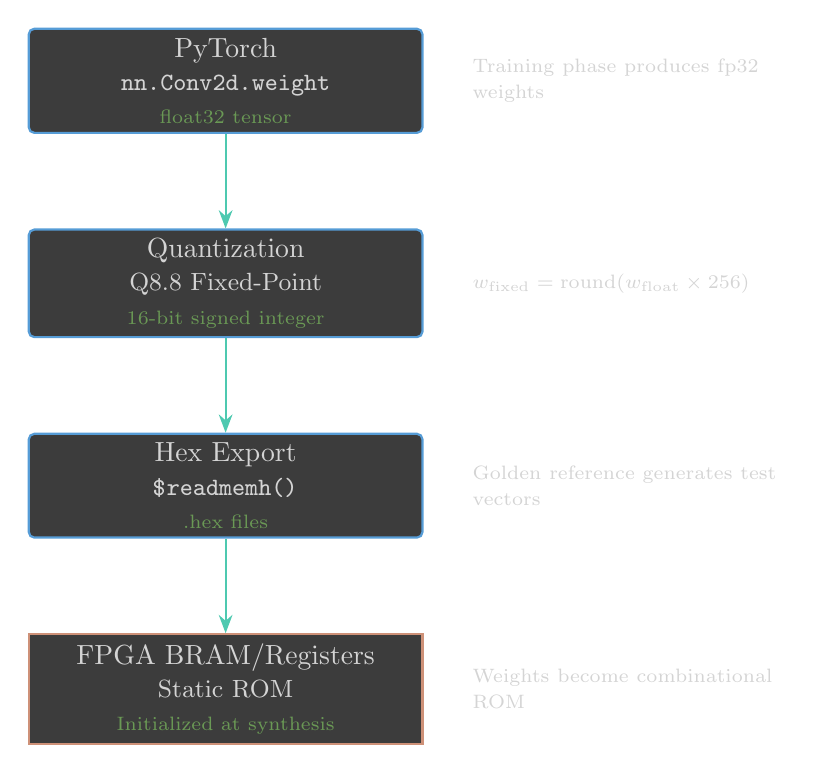
\begin{tikzpicture}[node distance=0.8cm]
    \node[block, minimum width=5cm] (pytorch) {PyTorch\\{\small\texttt{nn.Conv2d.weight}}\\{\scriptsize\color{codecomment}float32 tensor}};
    
    \node[block, minimum width=5cm, below=1.2cm of pytorch] (quantize) {Quantization\\{\small Q8.8 Fixed-Point}\\{\scriptsize\color{codecomment}16-bit signed integer}};
    
    \node[block, minimum width=5cm, below=1.2cm of quantize] (hexdump) {Hex Export\\{\small\texttt{\$readmemh()}}\\{\scriptsize\color{codecomment}.hex files}};
    
    \node[memblock, minimum width=5cm, below=1.2cm of hexdump] (bram) {FPGA BRAM/Registers\\{\small Static ROM}\\{\scriptsize\color{codecomment}Initialized at synthesis}};
    
    \draw[signal] (pytorch) -- (quantize);
    \draw[signal] (quantize) -- (hexdump);
    \draw[signal] (hexdump) -- (bram);
    
    \node[right=0.5cm of pytorch, label, text width=4cm] {\scriptsize Training phase produces fp32 weights};
    \node[right=0.5cm of quantize, label, text width=4cm] {\scriptsize $w_{\text{fixed}} = \text{round}(w_{\text{float}} \times 256)$};
    \node[right=0.5cm of hexdump, label, text width=4cm] {\scriptsize Golden reference generates test vectors};
    \node[right=0.5cm of bram, label, text width=4cm] {\scriptsize Weights become combinational ROM};
\end{tikzpicture}
\end{center}

The weights become \textbf{compile-time constants}---they do not change during inference. In Verilog, this manifests as:

\begin{lstlisting}[language=Verilog, caption={Weight ROM initialization pattern}]
reg signed [15:0] conv1_w [0:431];   // 16 outch * 3 inch * 9 taps = 432
reg signed [15:0] conv1_b [0:15];    // 16 biases

initial begin
    $readmemh("conv1_weights.hex", conv1_w);
    $readmemh("conv1_bias.hex", conv1_b);
end
\end{lstlisting}

On Xilinx FPGAs, the synthesis tool infers these as either:
\begin{itemize}[leftmargin=2em]
    \item \textbf{Distributed ROM}: Implemented in LUT memory for small arrays
    \item \textbf{Block RAM (BRAM)}: Dedicated 36Kb/18Kb memory primitives for larger arrays
\end{itemize}

\subsection{Layers: From Sequential Operations to Spatial Structures}

A PyTorch \texttt{nn.Conv2d} layer executes as millions of sequential multiply-accumulate operations on a GPU. In hardware, we have three architectural choices:

\begin{enumerate}[leftmargin=2em]
    \item \textbf{Fully Parallel}: Instantiate one multiplier per weight---maximum throughput, enormous area. A 3$\times$3$\times$16$\times$16 convolution would require $3 \times 3 \times 16 \times 16 = 2304$ multipliers.
    
    \item \textbf{Fully Sequential}: Single MAC unit, iterate through all taps---minimum area, maximum latency. Our \texttt{ldc\_block1} and \texttt{ldc\_block2} use this approach.
    
    \item \textbf{Hybrid}: Partial unrolling with multiple MACs---balance of throughput and area. Not implemented in this design.
\end{enumerate}

Our single-MAC architecture requires:
\begin{itemize}[leftmargin=2em]
    \item \textbf{27 cycles} per Conv1 output pixel in \texttt{ldc\_block1} (3 input channels $\times$ 9 taps)
    \item \textbf{144 cycles} per Conv2 output pixel in \texttt{ldc\_block1} (16 input channels $\times$ 9 taps)
    \item \textbf{144 cycles} per Conv1 output pixel in \texttt{ldc\_block2} (16 input channels $\times$ 9 taps)
    \item \textbf{288 cycles} per Conv2 output pixel in \texttt{ldc\_block2} (32 input channels $\times$ 9 taps)
\end{itemize}

\subsection{Activations: From Functions to Combinational Logic}

The ReLU activation function $f(x) = \max(0, x)$ becomes a single conditional operation:

\begin{lstlisting}[language=Verilog, caption={ReLU implementation via sign-bit inspection}]
// After bias addition and quantization shift:
// relu_result is the final Q8.8 output
if (relu_result[15])           // Sign bit check (negative?)
    relu_result = 16'sd0;      // Clamp to zero
\end{lstlisting}

This compiles to a simple 2:1 multiplexer controlled by the MSB---no comparator needed, just a sign-bit test followed by a conditional zero.

% =============================================================================
% CHAPTER 2: THE PYTHON GOLDEN REFERENCE
% =============================================================================

\chapter{The Python Golden Reference}

\section{Purpose: Software-Hardware Equivalence Verification}

Hardware verification is fundamentally a question of \textbf{equivalence}: does the RTL produce the same outputs as the reference model for all valid inputs? The Python Golden Reference serves as our \textit{oracle}---the authoritative source of correct behavior against which all hardware outputs are compared.

This approach addresses several challenges unique to CNN hardware:

\begin{enumerate}[leftmargin=2em]
    \item \textbf{No closed-form solution}: Unlike a simple ALU where $3 + 5 = 8$ can be verified by inspection, a 144-tap convolution has no ``obvious'' correct answer.
    
    \item \textbf{Quantization divergence}: Fixed-point arithmetic introduces rounding errors that compound through layers. The Python model must use \textit{identical} fixed-point operations, not floating-point approximations.
    
    \item \textbf{Intermediate observability}: The final output may be correct while intermediate values are wrong (compensating errors). The golden reference dumps \textit{every} intermediate value for cycle-accurate comparison.
\end{enumerate}

\section{Fixed-Point Arithmetic: Q8.8 and Q16.16}

Our design uses two fixed-point formats:

\begin{table}[h]
\centering
\begin{tabular}{@{}lcccc@{}}
\toprule
\textbf{Format} & \textbf{Bits} & \textbf{Integer} & \textbf{Fractional} & \textbf{Range} \\
\midrule
\qformat{Q8.8}  & 16 & 8 & 8 & $[-128.0, +127.996]$ \\
\qformat{Q16.16} & 32 & 16 & 16 & $[-32768.0, +32767.99998]$ \\
\bottomrule
\end{tabular}
\caption{Fixed-point format specifications}
\end{table}

\subsection{Q8.8: Input/Weight/Output Format}

The \qformat{Q8.8} format uses 16 signed bits with 8 fractional bits. The implicit scaling factor is $2^8 = 256$:

$$
\text{fixed\_value} = \text{round}(\text{float\_value} \times 256)
$$

$$
\text{float\_value} = \frac{\text{fixed\_value}}{256}
$$

In Python, the conversion functions mirror the Verilog testbench helpers:

\begin{lstlisting}[language=Python, caption={Python Q8.8 conversion functions}]
import numpy as np

def float_to_q88(f):
    """Convert float to Q8.8 (signed 16-bit)"""
    scaled = int(round(f * 256.0))
    # Clamp to signed 16-bit range
    return np.clip(scaled, -32768, 32767).astype(np.int16)

def q88_to_float(q):
    """Convert Q8.8 to float (for display)"""
    return float(np.int16(q)) / 256.0
\end{lstlisting}

\subsection{Q16.16: Accumulator Format}

Multiplication of two \qformat{Q8.8} values produces a \qformat{Q16.16} result (16 fractional bits from $8 + 8$). The accumulator must use this wider format to prevent overflow during the MAC chain:

\begin{lstlisting}[language=Python, caption={Q16.16 accumulation in Python}]
def mac_chain_q1616(pixels, weights):
    """
    Compute sum of products in Q16.16 format.
    pixels, weights: arrays of Q8.8 values (int16)
    Returns: Q16.16 accumulator value (int32)
    """
    accumulator = np.int32(0)
    for p, w in zip(pixels, weights):
        # Q8.8 * Q8.8 = Q16.16 (automatic in int32 multiply)
        product = np.int32(p) * np.int32(w)
        accumulator += product
    return accumulator
\end{lstlisting}

\subsection{Bias Addition and Requantization}

After accumulation, we add the bias (stored in \qformat{Q16.16} format) and requantize back to \qformat{Q8.8}:

\begin{lstlisting}[language=Python, caption={Bias, rounding, and ReLU}]
def bias_and_relu(accumulator, bias_q1616):
    """
    Add bias, round, shift, and apply ReLU.
    
    The +128 is the rounding constant for arithmetic right-shift:
    - We need to shift right by 8 to go from Q16.16 to Q8.8
    - Adding 0.5 LSB (128 in Q16.16 = 0.5 in the output Q8.8) 
      before shifting implements round-to-nearest
    """
    ROUNDING_CONSTANT = 128  # 0.5 LSB in Q16.16 relative to Q8.8 output
    
    biased = accumulator + bias_q1616 + ROUNDING_CONSTANT
    
    # Arithmetic right shift by 8 (Q16.16 -> Q8.8)
    # In Python, we use signed division; in Verilog, >>> operator
    shifted = biased >> 8  # Note: Python >> on negative is implementation-defined
    # Proper arithmetic shift:
    shifted = np.int32(biased) // 256  # Floor division handles sign correctly
    
    # ReLU: clamp negative to zero
    if shifted < 0:
        shifted = 0
    
    # Clamp to Q8.8 range (shouldn't be needed if architecture is correct)
    return np.clip(shifted, -32768, 32767).astype(np.int16)
\end{lstlisting}

\subsection{The Critical Rounding Constant: Why 32'sd128?}

The magic number \texttt{32'sd128} deserves careful explanation. When we right-shift by 8 bits, we are effectively dividing by 256. Integer division truncates toward zero (or toward negative infinity for arithmetic shift). To implement \textbf{round-to-nearest} instead:

$$
\text{round}(x / 256) = \lfloor (x + 128) / 256 \rfloor
$$

The value 128 is exactly half of 256---adding it before the shift means values $\geq 0.5$ LSB round up. In \qformat{Q16.16} terms, adding 128 adds $128 / 65536 \approx 0.00195$ to the accumulator, which becomes $0.5$ in the output \qformat{Q8.8} representation.

\section{Intermediate Value Dumping}

The golden reference generates hex files for every intermediate stage:

\begin{lstlisting}[language=Python, caption={Generating test vectors for hardware verification}]
def dump_intermediate_values(layer_name, values, filename):
    """
    Dump fixed-point values to hex file for $readmemh().
    Each line contains one 16-bit or 32-bit value in hexadecimal.
    """
    with open(filename, 'w') as f:
        for val in values.flatten():
            if isinstance(val, np.int16):
                # Q8.8: 16-bit, 4 hex digits
                f.write(f"{val & 0xFFFF:04X}\n")
            else:
                # Q16.16: 32-bit, 8 hex digits
                f.write(f"{val & 0xFFFFFFFF:08X}\n")
    print(f"[Golden Ref] Dumped {len(values.flatten())} values to {filename}")
\end{lstlisting}

For \texttt{ldc\_block1}, the golden reference produces:
\begin{itemize}[leftmargin=2em]
    \item \texttt{input\_image.hex}: 192 values (8$\times$8$\times$3 input pixels in \qformat{Q8.8})
    \item \texttt{conv1\_weights.hex}: 432 values (16 out $\times$ 3 in $\times$ 9 taps)
    \item \texttt{conv1\_bias.hex}: 16 values (16 output channels)
    \item \texttt{expected\_output.hex}: 256 values (4$\times$4$\times$16 output features)
\end{itemize}

% =============================================================================
% CHAPTER 3: HARDWARE ARCHITECTURE & RTL IMPLEMENTATION
% =============================================================================

\chapter{Hardware Architecture \& RTL Implementation}

This chapter details the core datapath elements, presenting the exact Verilog implementations with explanatory diagrams. All code excerpts are derived from the actual RTL as documented in the Elixir Summary.

\section{The Line Buffer \& 3$\times$3 Window Extraction}

\subsection{The Stream Processing Paradigm}

CNNs process images using \textbf{sliding window} convolutions: a 3$\times$3 kernel moves across the image, computing one output pixel per position. In software, this is typically implemented with nested loops accessing random memory locations. In hardware, we exploit the \textit{streaming} nature of pixel data.

Pixels arrive sequentially in raster-scan order (left-to-right, top-to-bottom). To compute a 3$\times$3 convolution at position $(r, c)$, we need simultaneous access to pixels at:

\begin{center}
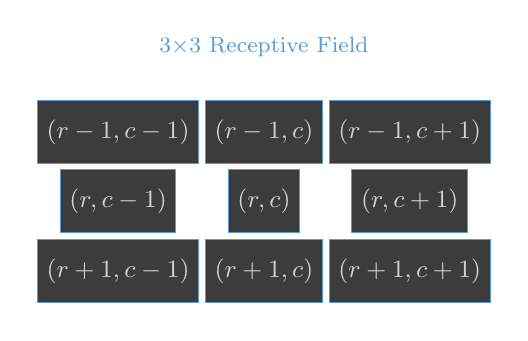
\begin{tikzpicture}
    \matrix[matrix of nodes, nodes={draw=blockborder, fill=blockfill, minimum size=0.8cm, text=textcolor, font=\small}, column sep=2pt, row sep=2pt] (window) {
        $(r-1,c-1)$ & $(r-1,c)$ & $(r-1,c+1)$ \\
        $(r,c-1)$   & $(r,c)$   & $(r,c+1)$ \\
        $(r+1,c-1)$ & $(r+1,c)$ & $(r+1,c+1)$ \\
    };
    \node[above=0.3cm of window, label, color=headingcolor] {3$\times$3 Receptive Field};
\end{tikzpicture}
\end{center}

The challenge: when pixel $(r+1, c+1)$ arrives, pixel $(r-1, c-1)$ was received $2 \times \text{IMG\_W} + 2$ clock cycles ago. We must buffer exactly this history.

\subsection{The Three-Row Shift Register Architecture}

The \texttt{line\_buffer} module implements a \textbf{3-row FIFO structure} using shift registers:

\begin{center}
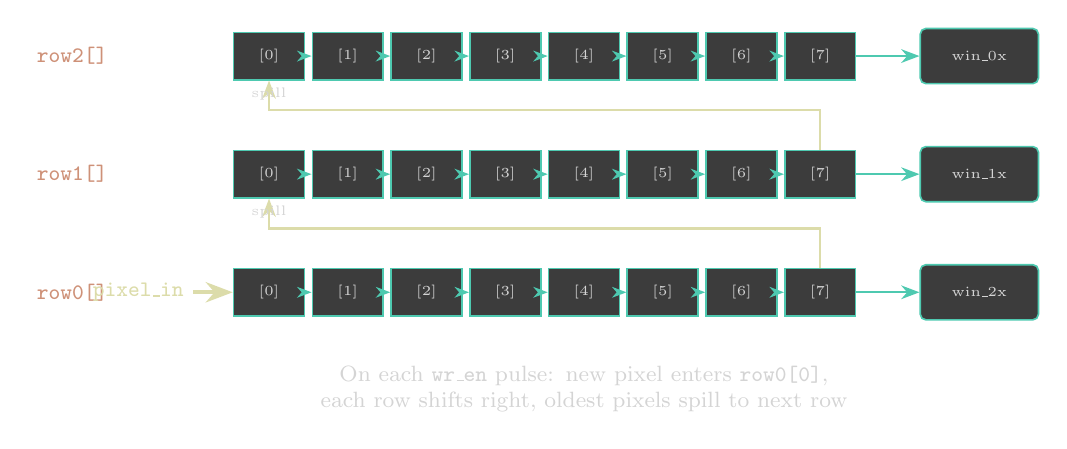
\begin{tikzpicture}[node distance=0.3cm]
    % Row labels
    \node[label, color=memorycolor] (r2label) at (-2.5, 0) {\texttt{row2[]}};
    \node[label, color=memorycolor] (r1label) at (-2.5, -1.5) {\texttt{row1[]}};
    \node[label, color=memorycolor] (r0label) at (-2.5, -3) {\texttt{row0[]}};
    
    % Row 2 (oldest - top)
    \foreach \i in {0,...,7} {
        \node[register, minimum width=0.9cm] (r2-\i) at (\i*1.0, 0) {\tiny[\i]};
    }
    
    % Row 1 (middle)
    \foreach \i in {0,...,7} {
        \node[register, minimum width=0.9cm] (r1-\i) at (\i*1.0, -1.5) {\tiny[\i]};
    }
    
    % Row 0 (newest - bottom, where pixel\_in enters)
    \foreach \i in {0,...,7} {
        \node[register, minimum width=0.9cm] (r0-\i) at (\i*1.0, -3) {\tiny[\i]};
    }
    
    % Shift arrows within rows
    \foreach \i in {1,...,7} {
        \pgfmathtruncatemacro{\prev}{\i-1}
        \draw[signal, line width=0.5pt] (r2-\prev.east) -- (r2-\i.west);
        \draw[signal, line width=0.5pt] (r1-\prev.east) -- (r1-\i.west);
        \draw[signal, line width=0.5pt] (r0-\prev.east) -- (r0-\i.west);
    }
    
    % Row spillover arrows
    \draw[data, line width=0.8pt] (r0-7.north) -- ++(0, 0.5) -| (r1-0.south) node[midway, above, label] {\tiny spill};
    \draw[data, line width=0.8pt] (r1-7.north) -- ++(0, 0.5) -| (r2-0.south) node[midway, above, label] {\tiny spill};
    
    % Input arrow
    \node[left=0.5cm of r0-0, label, color=datacolor] (pixin) {\texttt{pixel\_in}};
    \draw[bus] (pixin) -- (r0-0.west);
    
    % Window extraction (tapping from right side)
    \node[right=0.8cm of r2-7, smallblock, fill=blockfill, draw=accentcolor, minimum width=1.5cm] (tap2) {\tiny win\_0x};
    \node[right=0.8cm of r1-7, smallblock, fill=blockfill, draw=accentcolor, minimum width=1.5cm] (tap1) {\tiny win\_1x};
    \node[right=0.8cm of r0-7, smallblock, fill=blockfill, draw=accentcolor, minimum width=1.5cm] (tap0) {\tiny win\_2x};
    
    \draw[signal] (r2-7.east) -- (tap2.west);
    \draw[signal] (r1-7.east) -- (tap1.west);
    \draw[signal] (r0-7.east) -- (tap0.west);
    
    % Annotations
    \node[below=0.5cm of r0-4, label, text width=8cm, align=center] {
        \footnotesize On each \texttt{wr\_en} pulse: new pixel enters \texttt{row0[0]}, \\
        each row shifts right, oldest pixels spill to next row
    };
    
\end{tikzpicture}
\end{center}

\textbf{Key insight}: When a row fills completely, its rightmost element (the oldest pixel in that row) ``spills'' into position [0] of the next row. This creates a continuous 3-row history buffer.

\subsection{The Verilog Implementation}

\begin{lstlisting}[language=Verilog, caption={Line buffer shift register logic (actual RTL)}]
module line_buffer #(
    parameter IMG_W  = 8,
    parameter IMG_H  = 8,
    parameter DATA_W = 16
)(
    input  wire                 clk,
    input  wire                 rst_n,
    input  wire                 wr_en,
    input  wire [DATA_W-1:0]    pixel_in,
    
    // 3x3 window output (row-major: row 0 = oldest/top)
    output wire [DATA_W-1:0]    win_00, win_01, win_02,
    output wire [DATA_W-1:0]    win_10, win_11, win_12,
    output wire [DATA_W-1:0]    win_20, win_21, win_22
);
    // Three shift register rows
    reg [DATA_W-1:0] row0 [0:IMG_W-1];  // Newest (bottom)
    reg [DATA_W-1:0] row1 [0:IMG_W-1];  // Middle
    reg [DATA_W-1:0] row2 [0:IMG_W-1];  // Oldest (top)
    integer i;
    
    always @(posedge clk or negedge rst_n) begin
        if (!rst_n) begin
            for (i = 0; i < IMG_W; i = i + 1) begin
                row0[i] <= {DATA_W{1'b0}};
                row1[i] <= {DATA_W{1'b0}};
                row2[i] <= {DATA_W{1'b0}};
            end
        end 
        else if (wr_en) begin
            // Row 0: new pixel enters [0], shifts right
            row0[0] <= pixel_in;
            for (i = 1; i < IMG_W; i = i + 1) 
                row0[i] <= row0[i-1];
            
            // Row 1: row0's oldest pixel spills to [0]
            row1[0] <= row0[IMG_W-1];
            for (i = 1; i < IMG_W; i = i + 1) 
                row1[i] <= row1[i-1];
            
            // Row 2: row1's oldest pixel spills to [0]
            row2[0] <= row1[IMG_W-1];
            for (i = 1; i < IMG_W; i = i + 1) 
                row2[i] <= row2[i-1];
        end
    end
    
    // Window taps (rightmost 3 columns of each row)
    assign win_00 = row2[IMG_W-1];  assign win_01 = row2[IMG_W-2];  assign win_02 = row2[IMG_W-3];
    assign win_10 = row1[IMG_W-1];  assign win_11 = row1[IMG_W-2];  assign win_12 = row1[IMG_W-3];
    assign win_20 = row0[IMG_W-1];  assign win_21 = row0[IMG_W-2];  assign win_22 = row0[IMG_W-3];
endmodule
\end{lstlisting}

\subsection{Window Geometry: Understanding the Tap Positions}

The window outputs are combinational reads from the register arrays. For an 8-wide image:

\begin{itemize}[leftmargin=2em]
    \item \signal{win\_22} = \regname{row0[7]}: The most recently arrived pixel (after 8 shifts fill row0)
    \item \signal{win\_00} = \regname{row2[7]}: The oldest pixel in the window (arrived 24 cycles earlier)
\end{itemize}

The mapping \signal{win\_XY} corresponds to kernel position $(X, Y)$ where $X$ is the row (0=top, 2=bottom) and $Y$ is the column (0=left, 2=right).

\textbf{Critical timing}: A valid 3$\times$3 window first appears after:
\begin{itemize}[leftmargin=2em]
    \item 6 pushes to fill \regname{row0[5..7]} (the rightmost 3 taps)
    \item 8 more pushes to spill into \regname{row1} and fill positions [5..7]
    \item 8 more pushes to spill into \regname{row2} and fill positions [5..7]
    \item Total: $6 + 8 + 8 = 22$ pushes before all 9 window positions are from real data
\end{itemize}

In practice, for zero-padded convolutions, we begin reading the window earlier (padding contributes implicit zeros).

% -----------------------------------------------------------------------------

\section{The MAC Element (Multiply-Accumulate)}

\subsection{Combinational vs.\ Sequential: The Latency Trade-off}

A fundamental design decision in MAC units is whether the accumulation is:

\begin{enumerate}[leftmargin=2em]
    \item \textbf{Fully registered}: Each multiply-add takes one clock cycle. The accumulator is a flip-flop that updates every cycle. This maximizes clock frequency but introduces latency.
    
    \item \textbf{Combinational with registered output}: The multiply-add is combinational (happens within one clock period), but results are registered for timing closure. Our design uses this approach with a \textbf{2-stage pipeline}.
\end{enumerate}

\subsection{The Critical Combinational Tap}

Our \texttt{mac\_element} exposes both the registered output (\signal{acc\_out}) and a combinational tap (\signal{acc\_out\_comb}):

\begin{center}
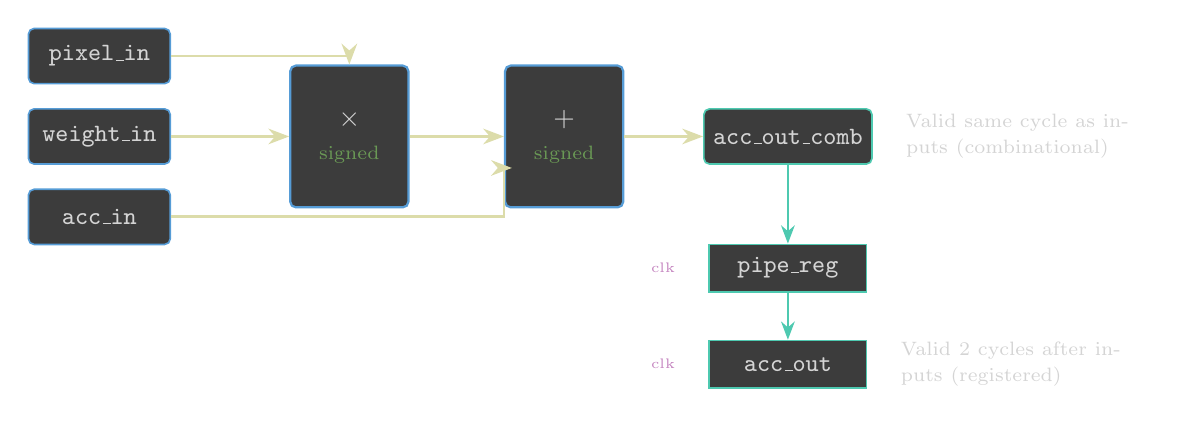
\begin{tikzpicture}[node distance=0.5cm]
    % Inputs
    \node[smallblock] (pixel) {\texttt{pixel\_in}};
    \node[smallblock, below=0.3cm of pixel] (weight) {\texttt{weight\_in}};
    \node[smallblock, below=0.3cm of weight] (accin) {\texttt{acc\_in}};
    
    % Multiplier
    \node[block, right=1.5cm of weight, minimum width=1.5cm, minimum height=1.8cm] (mult) {$\times$\\{\scriptsize\color{codecomment}signed}};
    
    % Adder
    \node[block, right=1.2cm of mult, minimum width=1.5cm, minimum height=1.8cm] (add) {+\\{\scriptsize\color{codecomment}signed}};
    
    % Combinational output
    \node[smallblock, right=1cm of add, fill=blockfill, draw=accentcolor] (combout) {\texttt{acc\_out\_comb}};
    
    % Pipeline registers
    \node[register, below=1cm of combout, minimum width=2cm] (pipe1) {\texttt{pipe\_reg}};
    \node[register, below=0.6cm of pipe1, minimum width=2cm] (pipe2) {\texttt{acc\_out}};
    
    % Connections
    \draw[data] (pixel.east) -| (mult.north);
    \draw[data] (weight.east) -- (mult.west);
    \draw[data] (mult.east) -- (add.west);
    \draw[data] (accin.east) -| ($(add.west)+(0,-0.4)$) -- ($(add.west)+(0.1,-0.4)$);
    \draw[data] (add.east) -- (combout.west);
    
    \draw[signal] (combout.south) -- (pipe1.north);
    \draw[signal] (pipe1.south) -- (pipe2.north);
    
    % Timing annotations
    \node[right=0.3cm of combout, label, text width=3cm] {\scriptsize Valid same cycle as inputs (combinational)};
    \node[right=0.3cm of pipe2, label, text width=3cm] {\scriptsize Valid 2 cycles after inputs (registered)};
    
    % Clock
    \node[left=0.3cm of pipe1, label, color=controlcolor] {\tiny clk};
    \node[left=0.3cm of pipe2, label, color=controlcolor] {\tiny clk};
    
\end{tikzpicture}
\end{center}

\textbf{Why the combinational tap matters}: In our FSM-driven architecture, the controller needs to chain MAC operations without inserting dead cycles. The combinational output \signal{acc\_out\_comb} allows the FSM to:
\begin{enumerate}[leftmargin=2em]
    \item Drive inputs for tap $k$ on clock edge $N$
    \item Read \signal{acc\_out\_comb} (the result including tap $k$) after the same clock edge
    \item Feed this back to \signal{acc\_in} for tap $k+1$
\end{enumerate}

Without this tap, we would need to wait 2 cycles per tap---a 2$\times$ throughput penalty.

\subsection{The Verilog Implementation}

\begin{lstlisting}[language=Verilog, caption={MAC element with combinational bypass (actual RTL)}]
module mac_element (
    input  wire        clk,
    input  wire        rst_n,
    input  wire        en,
    input  wire [15:0] pixel_in,    // Signed Q8.8
    input  wire [15:0] weight_in,   // Signed Q8.8
    input  wire [31:0] acc_in,      // Partial sum (Q16.16)
    output reg  [31:0] acc_out,     // Registered output (2-cycle latency)
    output wire [31:0] acc_out_comb // Combinational output (same-cycle)
);
    // Combinational multiply-add
    wire signed [31:0] w_product;
    assign w_product    = $signed(pixel_in) * $signed(weight_in);
    assign acc_out_comb = $signed(acc_in) + $signed(w_product);
    
    // 2-stage pipeline register
    reg [31:0] pipe_reg;
    
    always @(posedge clk or negedge rst_n) begin
        if (!rst_n) begin
            pipe_reg <= 32'sd0;
            acc_out  <= 32'sd0;
        end else if (en) begin
            pipe_reg <= acc_out_comb;  // Stage 1: capture combinational result
            acc_out  <= pipe_reg;       // Stage 2: final registered output
        end
    end
endmodule
\end{lstlisting}

\subsection{The \texttt{\$signed()} Directive}

Verilog treats \texttt{wire} and \texttt{reg} as unsigned by default. The \texttt{\$signed()} system function is essential for correct signed arithmetic:

\begin{itemize}[leftmargin=2em]
    \item \texttt{\$signed(pixel\_in) * \$signed(weight\_in)}: Performs a \textbf{signed multiplication}. Without this, $-1 \times 1$ would compute as $65535 \times 1 = 65535$ instead of $-1$.
    
    \item \texttt{\$signed(acc\_in) + \$signed(w\_product)}: Ensures sign extension during addition.
\end{itemize}

% -----------------------------------------------------------------------------

\section{\texttt{ldc\_block1}: The First Double Convolution Block}

\subsection{Architecture Overview}

\texttt{ldc\_block1} implements the first DoubleConvBlock:
\begin{itemize}[leftmargin=2em]
    \item \textbf{Input}: 8$\times$8 spatial, 3 channels (RGB), streamed pixel-by-pixel
    \item \textbf{Conv1}: 3$\times$3 kernel, stride-2, 16 output channels $\rightarrow$ 4$\times$4$\times$16 intermediate
    \item \textbf{Conv2}: 3$\times$3 kernel, stride-1, 16 output channels $\rightarrow$ 4$\times$4$\times$16 output
    \item \textbf{MAC counts}: 27 per Conv1 pixel (3$\times$9), 144 per Conv2 pixel (16$\times$9)
\end{itemize}

\begin{center}
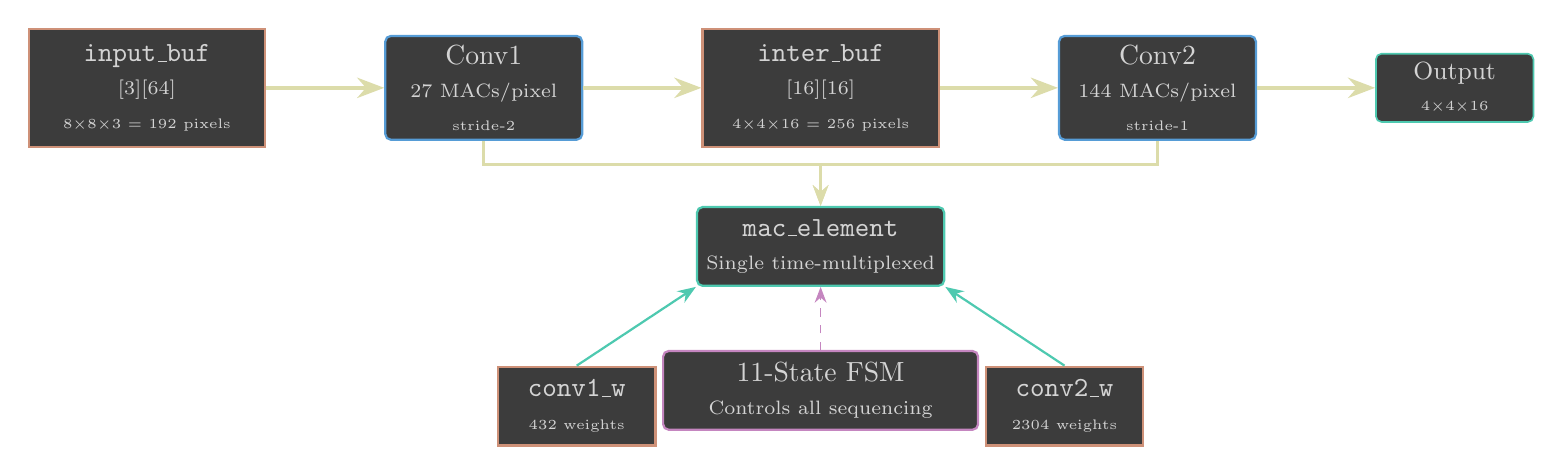
\begin{tikzpicture}[node distance=0.6cm]
    % Input buffer
    \node[memblock, minimum width=3cm, minimum height=1.5cm] (inbuf) {
        \texttt{input\_buf}\\
        {\scriptsize [3][64]}\\
        {\tiny 8$\times$8$\times$3 = 192 pixels}
    };
    
    % Conv1 processing
    \node[block, right=1.5cm of inbuf, minimum width=2.5cm] (conv1) {
        Conv1\\
        {\scriptsize 27 MACs/pixel}\\
        {\tiny stride-2}
    };
    
    % Intermediate buffer
    \node[memblock, right=1.5cm of conv1, minimum width=3cm, minimum height=1.5cm] (interbuf) {
        \texttt{inter\_buf}\\
        {\scriptsize [16][16]}\\
        {\tiny 4$\times$4$\times$16 = 256 pixels}
    };
    
    % Conv2 processing
    \node[block, right=1.5cm of interbuf, minimum width=2.5cm] (conv2) {
        Conv2\\
        {\scriptsize 144 MACs/pixel}\\
        {\tiny stride-1}
    };
    
    % Output
    \node[smallblock, right=1.5cm of conv2, minimum width=2cm, draw=accentcolor] (output) {
        Output\\
        {\tiny 4$\times$4$\times$16}
    };
    
    % MAC unit (shared)
    \node[block, below=1.5cm of $(conv1)!0.5!(conv2)$, minimum width=3cm, fill=blockfill, draw=accentcolor] (mac) {
        \texttt{mac\_element}\\
        {\scriptsize Single time-multiplexed}
    };
    
    % FSM
    \node[block, below=0.8cm of mac, minimum width=4cm, draw=controlcolor, fill=blockfill] (fsm) {
        11-State FSM\\
        {\scriptsize Controls all sequencing}
    };
    
    % Weight ROMs
    \node[memblock, below left=1cm and 0.5cm of mac, minimum width=2cm] (w1) {
        \texttt{conv1\_w}\\
        {\tiny 432 weights}
    };
    \node[memblock, below right=1cm and 0.5cm of mac, minimum width=2cm] (w2) {
        \texttt{conv2\_w}\\
        {\tiny 2304 weights}
    };
    
    % Data flow
    \draw[bus] (inbuf) -- (conv1);
    \draw[bus] (conv1) -- (interbuf);
    \draw[bus] (interbuf) -- (conv2);
    \draw[bus] (conv2) -- (output);
    
    % MAC connections
    \draw[data] (conv1.south) -- ++(0,-0.3) -| (mac.north);
    \draw[data] (conv2.south) -- ++(0,-0.3) -| (mac.north);
    
    % Weight connections
    \draw[signal] (w1.north) -- (mac.south west);
    \draw[signal] (w2.north) -- (mac.south east);
    
    % Control
    \draw[control] (fsm.north) -- (mac.south);
    
\end{tikzpicture}
\end{center}

\subsection{The 11-State FSM}

The FSM manages the complete inference pipeline:

\begin{enumerate}[leftmargin=2em]
    \item \state{S\_IDLE}: Wait for \signal{start} pulse
    \item \state{S\_LOAD\_INPUT}: Stream in 192 pixels (3 channels $\times$ 64 spatial positions)
    \item \state{S\_CONV1\_SETUP}: Initialize loop counters for Conv1
    \item \state{S\_CONV1\_MAC}: Execute 27 MAC operations per output pixel
    \item \state{S\_CONV1\_BIAS}: Add bias, requantize, apply ReLU, store to \regname{inter\_buf}
    \item \state{S\_CONV1\_NEXT}: Advance spatial/channel counters; loop or proceed
    \item \state{S\_CONV2\_SETUP}: Initialize loop counters for Conv2
    \item \state{S\_CONV2\_MAC}: Execute 144 MAC operations per output pixel
    \item \state{S\_CONV2\_BIAS}: Add bias, requantize, apply ReLU
    \item \state{S\_CONV2\_NEXT}: Advance counters; emit output with \signal{out\_pixel\_valid}
    \item \state{S\_DONE}: Assert \signal{block1\_ready}, return to \state{S\_IDLE}
\end{enumerate}

\subsection{Strided Convolution Index Math}

Conv1 uses stride-2, which means each output pixel $(out\_r, out\_c)$ reads from input positions centered at $(2 \times out\_r, 2 \times out\_c)$. The source coordinate calculation:

\begin{lstlisting}[language=Verilog, caption={Conv1 source coordinate calculation (stride-2)}]
// For kernel tap (kr, kc) where kr, kc in {0, 1, 2}:
wire signed [3:0] c1_src_r = ($signed({2'b00, out_r}) * 2) 
                           + $signed({2'b00, kr}) - 1;
wire signed [3:0] c1_src_c = ($signed({2'b00, out_c}) * 2) 
                           + $signed({2'b00, kc}) - 1;
\end{lstlisting}

The \texttt{- 1} implements zero-padding: when $out\_r = 0$ and $kr = 0$, we get $c1\_src\_r = 0 \times 2 + 0 - 1 = -1$, which maps to padding (returns 0).

\subsection{Weight ROM Addressing}

Weights are stored in a flat array with layout $[\text{out\_ch}][\text{in\_ch}][\text{tap}]$:

\begin{lstlisting}[language=Verilog, caption={Weight address calculation}]
// Conv1: 16 outch x 3 inch x 9 taps = 432 weights
wire [9:0] c1_w_addr = (out_ch * 27) + (mac_in_ch_wire[1:0] * 9) + mac_tap_wire;

// Conv2: 16 outch x 16 inch x 9 taps = 2304 weights  
wire [11:0] c2_w_addr = (out_ch * 144) + (mac_in_ch_wire * 9) + mac_tap_wire;
\end{lstlisting}

This matches PyTorch's default weight tensor ordering: \texttt{[out\_channels, in\_channels, kH, kW]}.

\subsection{The Combinational MAC Mux Pattern}

The critical performance optimization is the combinational feedback loop:

\begin{lstlisting}[language=Verilog, caption={Combinational MAC driving in FSM}]
// Combinational always block - drives MAC inputs
always @(*) begin
    mac_acc_in   = accumulator;            // Current partial sum
    mac_pixel_in = fetch_conv1_pixel(...); // Current pixel
    mac_weight   = conv1_w[c1_w_addr];     // Current weight
end

// Registered FSM - captures result and advances
always @(posedge clk or negedge rst_n) begin
    if (!rst_n) begin
        // Reset...
    end
    else case (state)
        S_CONV1_MAC: begin
            accumulator <= mac_acc_out_comb;  // Capture combinational result
            mac_cnt     <= mac_cnt + 1;        // Advance to next tap
            if (mac_cnt == 26)                 // Last tap?
                state <= S_CONV1_BIAS;
        end
        // ...
    endcase
end
\end{lstlisting}

This achieves \textbf{one MAC per clock cycle} despite the MAC element's 2-stage registered pipeline.

\subsection{Known Bugs in \texttt{ldc\_block1}}

The Elixir Summary documents two bugs in \texttt{ldc\_block1}:

\begin{enumerate}[leftmargin=2em]
    \item \textbf{Conv1 bias bug}: \state{S\_CONV1\_BIAS} incorrectly reads \texttt{conv2\_b[out\_ch]} instead of \texttt{conv1\_b[out\_ch]}. This silently applies Conv2 biases to Conv1 outputs, corrupting \regname{inter\_buf}.
    
    \item \textbf{\texttt{fetch\_conv2\_pixel} channel width bug}: The function parameter \texttt{[1:0] in\_ch\_f} can only index 4 channels, but Conv2 has 16 input channels. The 4-bit call argument is silently truncated. Additionally, the function reads from \regname{input\_buf} instead of \regname{inter\_buf}.
\end{enumerate}

These bugs are \textbf{fixed in \texttt{ldc\_block2}}.

% -----------------------------------------------------------------------------

\section{\texttt{ldc\_block2}: The Second Double Convolution Block}

\subsection{Dimensional Changes from Block1}

\begin{table}[h]
\centering
\begin{tabular}{@{}lcc@{}}
\toprule
\textbf{Parameter} & \textbf{Block1} & \textbf{Block2} \\
\midrule
Input dimensions & 8$\times$8$\times$3 & 4$\times$4$\times$16 \\
Output dimensions & 4$\times$4$\times$16 & 4$\times$4$\times$32 \\
Conv1 output channels & 16 & 32 \\
Conv2 output channels & 16 & 32 \\
MACs per Conv1 pixel & 27 (3$\times$9) & 144 (16$\times$9) \\
MACs per Conv2 pixel & 144 (16$\times$9) & 288 (32$\times$9) \\
\regname{mac\_cnt} width & \texttt{[7:0]} & \texttt{[8:0]} (288 needs 9 bits) \\
\regname{out\_ch} width & \texttt{[3:0]} & \texttt{[4:0]} (32 channels) \\
\texttt{conv1\_w} size & 432 & 4608 \\
\texttt{conv2\_w} size & 2304 & 9216 \\
\bottomrule
\end{tabular}
\caption{Dimensional comparison between Block1 and Block2}
\end{table}

\subsection{Stride-1 Throughout}

Both convolutions in Block2 use stride-1, preserving 4$\times$4 spatial resolution:

\begin{lstlisting}[language=Verilog, caption={Block2 source coordinate calculation (stride-1)}]
// Both Conv1 and Conv2 use identical stride-1 formula:
wire signed [3:0] c1_src_r = $signed({1'b0, out_r}) 
                           + $signed({1'b0, kr}) - 3'sd1;
wire signed [3:0] c1_src_c = $signed({1'b0, out_c}) 
                           + $signed({1'b0, kc}) - 3'sd1;

// Compare to Block1 Conv1 (stride-2):
// wire signed [3:0] c1_src_r = ($signed({2'b00, out_r}) * 2) + kr - 1;
\end{lstlisting}

\subsection{Input Loading Order Inversion}

Block1 loads pixels \textbf{channel-major}: all 64 pixels of channel 0, then channel 1, then channel 2.

Block2 loads pixels \textbf{pixel-major}: all 16 channels for pixel 0, then all 16 channels for pixel 1, etc.

\begin{lstlisting}[language=Verilog, caption={Block2 pixel-major loading (matches Block1 output order)}]
S_LOAD_INPUT: begin
    if (in_pixel_valid) begin
        input_buf[in_channel_idx][load_pixel_cnt] <= in_pixel_val;
        
        if (in_channel_idx == 4'd15) begin  // All channels for this pixel
            if (load_pixel_cnt == 4'd15)    // All pixels done
                state <= S_CONV1_SETUP;
            else
                load_pixel_cnt <= load_pixel_cnt + 1;
        end
        in_channel_idx <= in_channel_idx + 1;
    end
end
\end{lstlisting}

This matches Block1's output streaming order (Block1 emits \signal{out\_channel\_idx} incrementing fastest), enabling direct chaining without reordering buffers.

\subsection{Bug Fixes in Block2}

\begin{enumerate}[leftmargin=2em]
    \item \textbf{Conv1 bias fix}: \state{S\_CONV1\_BIAS} now correctly reads \texttt{conv1\_b[out\_ch]}.
    
    \item \textbf{\texttt{fetch\_conv2\_pixel} fix}: Function parameter expanded to \texttt{[4:0] in\_ch\_f}, reads from \regname{inter\_buf}, and bounds-checks against \texttt{MID\_H/MID\_W}.
\end{enumerate}

% =============================================================================
% CHAPTER 4: VERIFICATION, TESTING & DEBUGGING
% =============================================================================

\chapter{Verification, Testing \& Debugging Strategy}

\section{Testbench Architecture}

The verification strategy uses a \textbf{directed test} approach with golden reference comparison. Each testbench follows a common structure:

\begin{enumerate}[leftmargin=2em]
    \item \textbf{Initialization}: Load hex files (\texttt{\$readmemh}), reset DUT
    \item \textbf{Stimulus}: Drive inputs according to protocol (handshaking, timing)
    \item \textbf{Collection}: Capture outputs into memory arrays
    \item \textbf{Comparison}: Compare against expected values with tolerance
    \item \textbf{Reporting}: Count pass/fail, display diagnostics
\end{enumerate}

\subsection{Helper Functions for Q8.8 Verification}

\begin{lstlisting}[language=Verilog, caption={Testbench helper functions}]
// Float to Q8.8 conversion (for stimulus generation)
function [15:0] f2q88;
    input real f;
    begin
        f2q88 = $signed($rtoi(f * 256.0));
    end
endfunction

// Q16.16 to float conversion (for display)
function real q1616_to_real;
    input [31:0] q;
    begin
        q1616_to_real = $signed(q) / 65536.0;
    end
endfunction
\end{lstlisting}

\section{Race Conditions \& Reset Timing}

Simulation race conditions caused significant debugging effort. This section documents the specific issues and their fixes.

\subsection{The Asynchronous Reset Race}

\textbf{Problem}: Asserting reset on the same clock edge as data transitions creates a race between the reset path and the data path.

\textbf{Incorrect pattern}:
\begin{lstlisting}[language=Verilog, caption={Problematic reset timing}]
initial begin
    rst_n = 0;
    @(posedge clk);  // Reset releases ON the clock edge
    rst_n = 1;       // Race: does the register see reset or data?
    // ...
end
\end{lstlisting}

\textbf{Correct pattern (Block2 testbench)}:
\begin{lstlisting}[language=Verilog, caption={Glitch-free reset release on negedge}]
initial begin
    rst_n = 0;
    repeat(3) @(posedge clk);  // Hold reset for 3 cycles
    @(negedge clk);            // Release on negedge (mid-cycle)
    rst_n = 1;                 // Clean setup time for next posedge
    // ...
end
\end{lstlisting}

By releasing reset on the \textbf{negative edge}, we guarantee that the reset deassertion is stable long before the next positive edge samples it.

\subsection{The First-Pixel Drop Bug}

\textbf{Problem}: In \texttt{tb\_ldc\_block2}, the first input pixel was silently dropped.

\textbf{Root cause}: The testbench asserted \signal{start} and the first pixel simultaneously. The FSM transitioned from \state{S\_IDLE} to \state{S\_LOAD\_INPUT} on the clock edge, but the first pixel was presented on that same edge---before the FSM was ready to receive it.

\textbf{Fix}: Insert a guard cycle after start:
\begin{lstlisting}[language=Verilog, caption={Guard cycle fix for Block2}]
initial begin
    // ... reset sequence ...
    
    start = 1;
    @(posedge clk);
    start = 0;
    
    // CRITICAL: Wait one cycle for FSM to transition IDLE -> S_LOAD_INPUT
    @(posedge clk); #1;
    
    // Now safe to present first pixel
    stream_input_image();
end
\end{lstlisting}

\subsection{Non-Blocking Assignment Consistency}

All registered assignments must use non-blocking (\texttt{<=}) to avoid simulation/synthesis mismatches:

\begin{lstlisting}[language=Verilog, caption={Proper non-blocking usage in FSM}]
always @(posedge clk or negedge rst_n) begin
    if (!rst_n) begin
        pipe_reg <= 32'sd0;  // Non-blocking for reset
        acc_out  <= 32'sd0;
    end else if (en) begin
        pipe_reg <= acc_out_comb;  // Non-blocking for data
        acc_out  <= pipe_reg;
    end
end
\end{lstlisting}

\section{Success Criteria}

\subsection{\texttt{tb\_mac\_element}: 6 Test Cases}

\begin{table}[h]
\centering
\begin{tabular}{@{}clp{8cm}@{}}
\toprule
\textbf{Test} & \textbf{Name} & \textbf{Pass Criteria} \\
\midrule
T1 & Latency & \signal{acc\_out} = 0 at +1 cycle, correct at +2, stable at +3, frozen at +4 (\signal{en}=0) \\
T2 & Positive MAC & $1.5 \times 2.0 = 3.0$ $\rightarrow$ \texttt{0x00030000} exact match \\
T3 & Negative MAC & $1.5 \times (-2.0) = -3.0$ $\rightarrow$ \texttt{-32'sd196608} exact match \\
T4 & 9-tap chain & Sum of 9 products via \signal{acc\_out\_comb} feedback $\rightarrow$ 4.25 $\rightarrow$ \texttt{0x00044000} \\
T5 & Enable freeze & With \signal{en}=0, \signal{acc\_out} unchanged for 6 cycles despite new inputs \\
T6 & Mid-flight reset & Reset during pipeline $\rightarrow$ both post-reset cycles = 0 \\
\bottomrule
\end{tabular}
\caption{\texttt{tb\_mac\_element} test matrix}
\end{table}

\subsection{\texttt{tb\_line\_buffer}: 6 Test Cases}

\begin{table}[h]
\centering
\begin{tabular}{@{}clp{8cm}@{}}
\toprule
\textbf{Test} & \textbf{Name} & \textbf{Pass Criteria} \\
\midrule
T1 & Post-reset & All 9 window outputs = 0 \\
T2 & Window activation & \signal{win\_22} goes live at push 6; \signal{win\_00} stays 0 until row2 fills \\
T3 & Row spill & \regname{row1[5]} (\signal{win\_12}) non-zero at push 14 \\
T4 & Full window & After 26 pushes: exact pattern $\{3,4,5\}, \{11,12,13\}, \{19,20,21\}$ \\
T5 & Write disable & \signal{wr\_en}=0 with new data $\rightarrow$ all outputs frozen \\
T6 & 4-wide variant & 12 pushes on \texttt{dut2}: window = $\{1,2,3\}, \{5,6,7\}, \{9,10,11\}$ \\
\bottomrule
\end{tabular}
\caption{\texttt{tb\_line\_buffer} test matrix}
\end{table}

\subsection{\texttt{tb\_ldc\_block1}: Tolerance-Based Comparison}

\begin{itemize}[leftmargin=2em]
    \item \textbf{Input}: 192 pixels from \texttt{input\_image.hex}
    \item \textbf{Expected output}: 256 pixels from \texttt{expected\_output.hex}
    \item \textbf{Tolerance}: $\pm 1$ LSB (\qformat{Q8.8})
    \item \textbf{Pass}: \texttt{fail\_cnt == 0} across all 256 comparisons
\end{itemize}

\begin{lstlisting}[language=Verilog, caption={Block1 tolerance comparison}]
integer diff;

diff = $signed(captured_mem[idx]) - $signed(expected_mem[idx]);
if (diff < 0) diff = -diff;  // Absolute value

if (diff <= 1)
    pass_cnt = pass_cnt + 1;
else
    fail_cnt = fail_cnt + 1;
\end{lstlisting}

\subsection{\texttt{tb\_ldc\_block2}: Widened Tolerance}

Block2 uses $\pm 3$ LSB tolerance (vs.\ $\pm 1$ for Block1) because:
\begin{itemize}[leftmargin=2em]
    \item Longer MAC chains (144/288 taps vs.\ 27/144)
    \item Accumulated rounding errors from the \texttt{+128} constant
    \item Block1 output (Block2's input) already has $\pm 1$ error
\end{itemize}

\subsection{Timing Budgets}

\begin{table}[h]
\centering
\begin{tabular}{@{}lcc@{}}
\toprule
\textbf{Testbench} & \textbf{Expected Cycles} & \textbf{Watchdog Timeout} \\
\midrule
\texttt{tb\_ldc\_block1} & $\sim$45,512 & 10 ms (1,000,000 cycles @ 100 MHz) \\
\texttt{tb\_ldc\_block2} & $>$100,000 & 20 ms (2,000,000 cycles @ 100 MHz) \\
\bottomrule
\end{tabular}
\caption{Simulation timing parameters}
\end{table}

\textbf{Vivado note}: The default xsim runtime of 1000 ns is insufficient. Use \texttt{-all} flag or explicit \texttt{run -all} command.

% =============================================================================
% APPENDIX: QUICK REFERENCE
% =============================================================================

\appendix
\chapter{Quick Reference}

\section{Fixed-Point Format Summary}

\begin{table}[h]
\centering
\begin{tabular}{@{}llll@{}}
\toprule
\textbf{Signal Type} & \textbf{Format} & \textbf{Bits} & \textbf{Example Conversion} \\
\midrule
Input pixels & \qformat{Q8.8} & 16 signed & $1.5 \rightarrow 384$ (0x0180) \\
Weights & \qformat{Q8.8} & 16 signed & $-0.5 \rightarrow -128$ (0xFF80) \\
Biases & \qformat{Q16.16} & 32 signed & $0.5 \rightarrow 32768$ (0x00008000) \\
Accumulator & \qformat{Q16.16} & 32 signed & $3.0 \rightarrow 196608$ (0x00030000) \\
Output pixels & \qformat{Q8.8} & 16 signed & After shift and ReLU \\
\bottomrule
\end{tabular}
\end{table}

\section{State Machine Quick Reference}

\textbf{Block1/Block2 State Progression}:

\begin{center}
\state{S\_IDLE} $\rightarrow$ \state{S\_LOAD\_INPUT} $\rightarrow$ \state{S\_CONV1\_SETUP} $\rightarrow$ \state{S\_CONV1\_MAC} $\rightarrow$ \state{S\_CONV1\_BIAS} $\rightarrow$ \state{S\_CONV1\_NEXT} $\rightarrow$ \\[0.3em]
$\rightarrow$ \state{S\_CONV2\_SETUP} $\rightarrow$ \state{S\_CONV2\_MAC} $\rightarrow$ \state{S\_CONV2\_BIAS} $\rightarrow$ \state{S\_CONV2\_NEXT} $\rightarrow$ \state{S\_DONE}
\end{center}

\section{Key Equations}

\textbf{MAC operation}:
$$
\text{acc\_out\_comb} = \text{acc\_in} + (\text{pixel\_in} \times \text{weight\_in})
$$

\textbf{Bias and quantization}:
$$
\text{relu\_result} = \max\left(0, \left\lfloor \frac{\text{accumulator} + \text{bias} + 128}{256} \right\rfloor\right)
$$

\textbf{Stride-2 source coordinate} (Block1 Conv1):
$$
\text{src\_r} = 2 \times \text{out\_r} + \text{kr} - 1
$$

\textbf{Stride-1 source coordinate} (Block1 Conv2, Block2 Conv1/Conv2):
$$
\text{src\_r} = \text{out\_r} + \text{kr} - 1
$$

\textbf{Weight address}:
$$
\text{addr} = (\text{out\_ch} \times \text{taps\_per\_out\_ch}) + (\text{in\_ch} \times 9) + \text{tap}
$$

\begin{figure}[htbp]
    \centering
    
    % --- TOP ROW ---
    \begin{minipage}{0.48\textwidth}
        \centering
        
\includegraphics[width=\linewidth]{C:/Users/rahul/LDC/data/35028.jpg}
        \par\vspace{0.2em} (a) Original Image
    \end{minipage}\hfill
    \begin{minipage}{0.48\textwidth}
        \centering
        
\includegraphics[width=\linewidth]{C:/Users/rahul/LDC/result/BIPED2CLASSIC/fused/35028.png}
        \par\vspace{0.2em} (b) LDC Output (Ours)
    \end{minipage}

    \vspace{1.5em} % Spacing between the rows

    % --- BOTTOM ROW ---
    \begin{minipage}{0.48\textwidth}
        \centering
        \includegraphics[width=\linewidth]{C:/Users/rahul/result_sobel_raw.png}
        \par\vspace{0.2em} (c) Traditional Sobel
    \end{minipage}\hfill
    \begin{minipage}{0.48\textwidth}
        \centering
        \includegraphics[width=\linewidth]{C:/Users/rahul/canny_output.png}
        \par\vspace{0.2em} (d) Traditional Canny
    \end{minipage}

    \caption{Qualitative evaluation of edge detection algorithms. The traditional Sobel (c) and Canny (d) operators capture unwanted high-frequency background noise. In contrast, the learned parameters of the LDC architecture (b) successfully isolate clean, semantic object boundaries.}
    \label{fig:edge_comparison_grid}
\end{figure}

\section{2D Convolution Line Buffer Datapath and Window Generation}

This section specifies the microarchitectural implementation of the line buffer datapath and sliding window generation logic employed by the Lightweight Dense CNN (LDC) edge detection accelerator. The module ingests a raster-scanned pixel stream and produces nine simultaneous spatial taps for a $3 \times 3$ convolution kernel. Correct understanding of the temporal-to-spatial mapping, shift register indexing conventions, and pipeline latency is essential for RTL verification and timing closure.

% ------------------------------------------------------------------------------
\subsection{Hardware Streaming Mechanics and the Right-to-Left Shift Architecture}

\subsubsection{Raster Scan Input Protocol}

The upstream image source transmits pixels in strict raster scan order: left-to-right across each row, top-to-bottom across rows. For an image of width $\mathtt{IMGW} = 8$, the chronological arrival sequence is:

\begin{center}
\texttt{A1 $\rightarrow$ A2 $\rightarrow$ \ldots $\rightarrow$ A8 $\rightarrow$ B1 $\rightarrow$ \ldots $\rightarrow$ B8 $\rightarrow$ C1 $\rightarrow$ \ldots $\rightarrow$ C8}
\end{center}

Each pixel arrives on the rising edge of the system clock and is pushed into the head of the shift register fabric.

\subsubsection{Shift Register Fabric Topology}

The line buffer comprises three discrete shift register rows declared in Verilog as:

\begin{verbatim}
    reg [DATAWIDTH-1:0] row0 [7:0];
    reg [DATAWIDTH-1:0] row1 [7:0];
    reg [DATAWIDTH-1:0] row2 [7:0];
\end{verbatim}

The array index convention follows standard Verilog semantics where the \emph{higher} index denotes the \emph{leftmost} (entry) position:

\begin{itemize}[leftmargin=2em]
    \item \textbf{Index [7]} --- Entry node (MSB end). New pixels are inserted here.
    \item \textbf{Index [0]} --- Exit node (LSB end). Oldest resident pixel; spillover source.
\end{itemize}

On every clock edge, the shift operation moves data \emph{toward lower indices}:

\begin{verbatim}
    row0[6:0] <= row0[7:1];   // Shift right (toward index 0)
    row0[7]   <= pixelin;    // New pixel enters at index 7
\end{verbatim}

\subsubsection{Resolving the Temporal--Spatial Layout Paradox}

A frequent source of RTL bugs arises from conflating \emph{temporal arrival order} with \emph{spatial array layout}. The key insight is:

\begin{quote}
\emph{The newest pixel occupies the highest index; the oldest pixel occupies the lowest index. Data flows from high indices toward low indices on each clock cycle.}
\end{quote}

When visualizing the shift register as a horizontal structure, index [7] sits at the \textbf{left} (entry) and index [0] at the \textbf{right} (exit). Pixels therefore appear to shift \emph{rightward} through the array, despite arriving in left-to-right image order. This inversion is intentional and aligns the convolution window taps with spatially contiguous image columns.

\subsubsection{Inter-Row Cascade (Spillover) Connections}

The three rows are daisy-chained via hardwired spillover connections:

\begin{itemize}[leftmargin=2em]
    \item \texttt{row0}[0] $\rightarrow$ \texttt{row1}[7] (on next clock edge)
    \item \texttt{row1}[0] $\rightarrow$ \texttt{row2}[7] (on next clock edge)
\end{itemize}

This cascade ensures that after $\mathtt{IMGW} = 8$ clock cycles, the oldest pixel in \texttt{row0} spills into the entry position of \texttt{row1}, and similarly for \texttt{row1} into \texttt{row2}. The total fabric depth is $3 \times 8 = 24$ pixel slots.

% ------------------------------------------------------------------------------
\subsection{Visual Pipelining Steps: Push Trace Analysis}

The following trace diagrams illustrate the exact contents of each shift register slot at critical pipeline milestones. All unlabeled positions contain the initial value of zero (denoted by \texttt{--}). Pixel labels use the notation $\langle\mathit{Row}\rangle\langle\mathit{Column}\rangle$ (e.g., \texttt{A3} is row A, column 3).

\subsubsection{Milestone 1: Push 6 --- First Partial Row Loaded}

After six clock cycles, six pixels from Line A occupy positions [7:2] of \texttt{row0}. The entry window taps [7:5] now contain valid data (\texttt{A6}, \texttt{A5}, \texttt{A4}), but only from a single image row.

\begin{verbatim}
             Index:   [7]   [6]   [5]   [4]   [3]   [2]   [1]   [0]
            --------------------------------------------------------
            row0:     A6    A5    A4    A3    A2    A1    --    --
            row1:     --    --    --    --    --    --    --    --
            row2:     --    --    --    --    --    --    --    --
\end{verbatim}

\textbf{Observation:} The window taps [7:5] across all three rows do not yet span three distinct image rows; \texttt{valid\_out} remains deasserted.

\subsubsection{Milestone 2: Push 14 --- Two Rows Populated}

After 14 pushes, Line A has completely traversed \texttt{row0} and partially filled \texttt{row1}. Line B occupies \texttt{row0}[7:2]. The cascade connection has transferred \texttt{A8} through \texttt{A3} into \texttt{row1}.

\begin{verbatim}
             Index:   [7]   [6]   [5]   [4]   [3]   [2]   [1]   [0]
            --------------------------------------------------------
            row0:     B6    B5    B4    B3    B2    B1    A8    A7
            row1:     A6    A5    A4    A3    A2    A1    --    --
            row2:     --    --    --    --    --    --    --    --
\end{verbatim}

\textbf{Observation:} Window taps now span two image rows (B and A), but \texttt{row2} remains empty. The $3 \times 3$ window is still incomplete.

\subsubsection{Milestone 3: Push 22 --- Valid Window Alignment}

After 22 pushes, the pipeline reaches first valid output. Line C has advanced six positions into \texttt{row0}, Line B fully populates the tap region of \texttt{row1}, and Line A occupies the tap region of \texttt{row2}.

\begin{verbatim}
             Index:   [7]   [6]   [5]   [4]   [3]   [2]   [1]   [0]
            --------------------------------------------------------
            row0:     C6    C5    C4    C3    C2    C1    B8    B7
            row1:     B6    B5    B4    B3    B2    B1    A8    A7
            row2:     A6    A5    A4    A3    A2    A1    --    --
\end{verbatim}

\textbf{Critical Timing Rationale:} Although \texttt{row2}[1:0] remain unpopulated, the convolution taps are wired exclusively to indices [7:5]. At push 22:

\begin{itemize}[leftmargin=2em]
    \item \texttt{row0}[7:5] = \{\texttt{C6}, \texttt{C5}, \texttt{C4}\}
    \item \texttt{row1}[7:5] = \{\texttt{B6}, \texttt{B5}, \texttt{B4}\}
    \item \texttt{row2}[7:5] = \{\texttt{A6}, \texttt{A5}, \texttt{A4}\}
\end{itemize}

These nine values form a spatially coherent $3 \times 3$ patch centered at image coordinate $(5, \mathrm{B})$---the earliest valid convolution site. Deferring until push 24 would shift \texttt{A4} past the tap window, corrupting horizontal alignment.

The latency formula for first valid output is:

$$
L_{\mathrm{valid}} = 2 \cdot \mathtt{IMGW} + (\mathtt{KERNEL\_WIDTH} - 1 + 3) = 2 \cdot 8 + 6 = 22 \text{ cycles}
$$

% ------------------------------------------------------------------------------
\subsection{Window Geometry Mapping and Spatial Inversion Safety}

\subsubsection{Tap-to-Window Coordinate Assignment}

The nine convolution taps are extracted from fixed indices [7], [6], and [5] of each row. The mapping to kernel matrix positions $\mathbf{W}$ follows the convention where row index increases downward (toward older image lines) and column index increases leftward (toward newer pixels within a row):

\begin{table}[htbp]
\centering
\caption{Window Tap Mapping to Shift Register Indices}
\begin{tabular}{@{}lcccc@{}}
\toprule
\textbf{Kernel Position} & \textbf{Signal} & \textbf{Source Register} & \textbf{Image Row} & \textbf{Relative Column} \\
\midrule
$\mathbf{W}[0][0]$ & \texttt{win00} & \texttt{row2}[7] & Oldest (A) & Left \\
$\mathbf{W}[0][1]$ & \texttt{win01} & \texttt{row2}[6] & Oldest (A) & Center \\
$\mathbf{W}[0][2]$ & \texttt{win02} & \texttt{row2}[5] & Oldest (A) & Right \\
\midrule
$\mathbf{W}[1][0]$ & \texttt{win10} & \texttt{row1}[7] & Middle (B) & Left \\
$\mathbf{W}[1][1]$ & \texttt{win11} & \texttt{row1}[6] & Middle (B) & Center \\
$\mathbf{W}[1][2]$ & \texttt{win12} & \texttt{row1}[5] & Middle (B) & Right \\
\midrule
$\mathbf{W}[2][0]$ & \texttt{win20} & \texttt{row0}[7] & Newest (C) & Left \\
$\mathbf{W}[2][1]$ & \texttt{win21} & \texttt{row0}[6] & Newest (C) & Center \\
$\mathbf{W}[2][2]$ & \texttt{win22} & \texttt{row0}[5] & Newest (C) & Right \\
\bottomrule
\end{tabular}
\end{table}

\subsubsection{Row Mapping Rationale: Freshest Data in \texttt{row0}}

A common verification pitfall is the assumption that \texttt{row0} corresponds to the \emph{topmost} image row. In a streaming architecture, the opposite holds:

\begin{itemize}[leftmargin=2em]
    \item \texttt{row0} contains the \textbf{most recently arrived} image row (youngest data).
    \item \texttt{row2} contains the \textbf{earliest arrived} image row (oldest data).
\end{itemize}

When the convolution kernel coefficients are defined with index [0][*] representing the top row of the filter (as is conventional in image processing), the hardware must map \texttt{row2}~$\rightarrow$~kernel row 0, \texttt{row1}~$\rightarrow$~kernel row 1, and \texttt{row0}~$\rightarrow$~kernel row 2. Failure to invert this mapping produces a vertically mirrored convolution result.

\subsubsection{Off-by-One and Mirror-Inversion Bug Patterns}

RTL designers should guard against the following common errors:

\begin{enumerate}[leftmargin=2em]
    \item \textbf{Horizontal Mirror Inversion} --- Swapping the column tap order (e.g., \texttt{row0}[5] assigned to \texttt{win20} instead of \texttt{win22}) inverts the kernel horizontally. For symmetric filters (e.g., Sobel-X), this may silently negate the gradient sign.

    \item \textbf{Vertical Mirror Inversion} --- Mapping \texttt{row0} to kernel row 0 instead of kernel row 2 inverts the vertical axis. Edge-detection kernels will report gradients in the opposite direction.

    \item \textbf{Premature Valid Assertion} --- Asserting \texttt{valid\_out} before push 22 (for $\mathtt{IMGW} = 8$) exposes incomplete rows to the MAC tree. Simulation with a known impulse image can diagnose this by checking that the first output corresponds to the expected spatial coordinate.

    \item \textbf{Tap Index Drift} --- Using parameterized tap indices without accounting for \texttt{IMGW} changes. The general formula for the rightmost tap index is $\mathtt{IMGW} - \mathtt{KERNEL\_WIDTH} = 8 - 3 = 5$, not a hardcoded constant.
\end{enumerate}

\subsubsection{Verification Recommendations}

\begin{itemize}[leftmargin=2em]
    \item Inject a unit impulse image (single nonzero pixel) and verify that the output response matches the expected kernel coefficient at the correct output coordinate.

    \item Compare RTL simulation against a bit-accurate C/Python reference model operating on identical input streams with identical fixed-point representations (e.g., Q8.8).

    \item Assert formal properties on \texttt{valid\_out} to guarantee it remains deasserted for exactly $L_{\mathrm{valid}} - 1$ cycles after reset.

    \item Use constrained-random testing with asymmetric kernels to expose horizontal or vertical mirroring defects that symmetric kernels would mask.
\end{itemize}
% =============================================================================
% END DOCUMENT
% =============================================================================
\begin{tikzpicture}[
    cell/.style={draw, minimum width=1.1cm, minimum height=0.8cm, font=\footnotesize\ttfamily},
    cascade/.style={->, >=stealth, thick, red!70!black},
    shift/.style={->, >=stealth, gray, thick},
    tap/.style={dashed, blue!60!black, thick},
    label/.style={font=\small\bfseries}
]

% ===== ROW 0 (Newest Data) =====
\node[label] at (-1.5, 0) {\regname{row0}};
\foreach \i/\col in {0/white, 1/white, 2/white, 3/white, 4/white, 5/green!15, 6/green!15, 7/green!15} {
    \node[cell, fill=\col] (r0c\i) at ({(7-\i)*1.2}, 0) {[\i]};
}
\node[font=\scriptsize, above=0.1cm of r0c7] {Data In};
\draw[cascade, line width=1.5pt] ($(r0c7.north)+(0,0.4)$) -- (r0c7.north);

% Shift arrows within row0
\foreach \i in {1,...,7} {
    \pgfmathtruncatemacro{\prev}{\i-1}
    \draw[shift] (r0c\i.east) -- (r0c\prev.west);
}

% ===== ROW 1 (Middle Data) =====
\node[label] at (-1.5, -1.5) {\regname{row1}};
\foreach \i/\col in {0/white, 1/white, 2/white, 3/white, 4/white, 5/green!15, 6/green!15, 7/green!15} {
    \node[cell, fill=\col] (r1c\i) at ({(7-\i)*1.2}, -1.5) {[\i]};
}

% Shift arrows within row1
\foreach \i in {1,...,7} {
    \pgfmathtruncatemacro{\prev}{\i-1}
    \draw[shift] (r1c\i.east) -- (r1c\prev.west);
}

% ===== ROW 2 (Oldest Data) =====
\node[label] at (-1.5, -3) {\regname{row2}};
\foreach \i/\col in {0/white, 1/white, 2/white, 3/white, 4/white, 5/green!15, 6/green!15, 7/green!15} {
    \node[cell, fill=\col] (r2c\i) at ({(7-\i)*1.2}, -3) {[\i]};
}

% Shift arrows within row2
\foreach \i in {1,...,7} {
    \pgfmathtruncatemacro{\prev}{\i-1}
    \draw[shift] (r2c\i.east) -- (r2c\prev.west);
}

% ===== CASCADE CONNECTIONS =====
\draw[cascade, line width=1.5pt] 
    (r0c0.south) -- ++(0,-0.25) -| ($(r1c7.north)+(0.3,0)$) -- (r1c7.north);
\draw[cascade, line width=1.5pt] 
    (r1c0.south) -- ++(0,-0.25) -| ($(r2c7.north)+(0.3,0)$) -- (r2c7.north);

% ===== WINDOW TAP BOX =====
\draw[tap, rounded corners=3pt] 
    ($(r0c7.north west)+(-0.15,0.15)$) rectangle ($(r2c5.south east)+(0.15,-0.15)$);
\node[font=\scriptsize\bfseries, blue!60!black, above right] 
    at ($(r0c5.north east)+(0.2,0.2)$) {3×3 Window Taps};

% ===== OUTPUT SIGNALS =====
\node[font=\scriptsize\ttfamily, right=0.3cm of r0c5] (w00) {\signal{win\_00}};
\node[font=\scriptsize\ttfamily, right=0.3cm of r0c6] (w01) {\signal{win\_01}};
\node[font=\scriptsize\ttfamily, right=0.3cm of r0c7] (w02) {\signal{win\_02}};

\draw[->, >=stealth, blue!50] (r0c5.east) -- (w00.west);
\draw[->, >=stealth, blue!50] (r0c6.east) -- (w01.west);
\draw[->, >=stealth, blue!50] (r0c7.east) -- (w02.west);

\node[font=\scriptsize\ttfamily, right=0.3cm of r1c5] (w10) {\signal{win\_10}};
\node[font=\scriptsize\ttfamily, right=0.3cm of r1c6] (w11) {\signal{win\_11}};
\node[font=\scriptsize\ttfamily, right=0.3cm of r1c7] (w12) {\signal{win\_12}};

\draw[->, >=stealth, blue!50] (r1c5.east) -- (w10.west);
\draw[->, >=stealth, blue!50] (r1c6.east) -- (w11.west);
\draw[->, >=stealth, blue!50] (r1c7.east) -- (w12.west);

\node[font=\scriptsize\ttfamily, right=0.3cm of r2c5] (w20) {\signal{win\_20}};
\node[font=\scriptsize\ttfamily, right=0.3cm of r2c6] (w21) {\signal{win\_21}};
\node[font=\scriptsize\ttfamily, right=0.3cm of r2c7] (w22) {\signal{win\_22}};

\draw[->, >=stealth, blue!50] (r2c5.east) -- (w20.west);
\draw[->, >=stealth, blue!50] (r2c6.east) -- (w21.west);
\draw[->, >=stealth, blue!50] (r2c7.east) -- (w22.west);

% ===== LEGEND =====
\node[anchor=north west, font=\scriptsize] at (0, -4.2) {
    \textcolor{red!70!black}{\textbf{→}} Cascade Path \quad
    \textcolor{gray}{\textbf{→}} Shift Direction \quad
    \textcolor{green!40!black}{\rule{0.4cm}{0.3cm}} Window Tap Region
};

\end{tikzpicture}

\end{document}
